\documentclass[sigconf]{acmart}

\settopmatter{printacmref=false}
 
%\usepackage{cite} % will order citations
\usepackage{latexsym}
\usepackage{url}
\usepackage{xspace}
\usepackage{setspace}
\usepackage{color}
\usepackage{mdframed}
\usepackage{algorithm}
\usepackage{algpseudocode}
\usepackage{amsmath} 
\usepackage{natbib}
%\usepackage{amssymb}
\usepackage{amsthm}

\usepackage{graphicx}



\author{Camilo Tello Fachin 12127084}
\affiliation{
  \institution{TU Wien (Computational Science \& Engineering)}
  \city{Vienna}
  \country{Austria}
}
\email{e12127084@student.tuwien.ac.at}

\setcopyright{none}
%\copyrightyear{2024}
\acmYear{}
\acmDOI{}
\acmISBN{}
\acmConference{Seminar on Algorithms/Software Engineering}{WS 2023/24}{Vienna}
\acmBooktitle{}
\acmPrice{}

\title{Seminar summary of ``Interval Coloring of Stencil Graphs''}

\begin{document}

\maketitle

\section{Abstract} 
The paper 'Coloring the Vertices of 9-pt and 27-pt Stencils with Intervals' by D. Durrman
and E. Saule \cite{main_paper} is the subject of this summary which is done in the context of the seminar in Algorithms/Software 
Engineering Winter Semester 2023/24 at TU Vienna. In essence, the authors used graph theory 
to schedule parallel tasks which they then executed according to the found solution of 
their graph problem. They successfully derived and proved upper bounds for their algorithms, 
the most relevant of which is the bipartite decomposition for 2D stencils, which is at most 
twice as slow or less efficient as the optimal solution of the problem. The authors extended 
also to the 3D stencils where they arrived at an upper bound of their solution being up 
to 4 times slower or less efficient than the optimal solution. They successfully used their 
algorithm on the space-time-kernel density estimation to obtain faster solutions to this 
known data processing problem which benefits vastly from parallelization of subtasks which 
are not adjacent to each other in space and time, see \cite{kernel_estimation_1} and \cite{kernel_estimation_2}. In order to find the true solution qualities 
of their algorithms, they solved a large part of the problems with an Integer Program to 
obtain optimal solutions. For their best algorithm, Bipartite Decomposition + Post, 95\% 
of the solved instances were at most 20\% worse than the best solution. The + Post part 
being a greedy procedure recoloring each vertex if neighbors admit it.

\section{Introduction}
For a given parallel processing problem, one can model processing tasks that cannot be computed
at the same time with 2 vertices connected by an edge. For a large problem, the simple solution is to
solve the $\textsc{Vertex Coloring Problem}$ of an undirected graph $G(V,E)$. Suppose the single tasks have different 
computational intensity, i.e. take varying amout of time for completion, the classical vertex coloring
problem is rendered suboptimal since it will most certainly introduce idling times during parallel
execution. The $\textsc{Interval Vertex Coloring Problem}$ or short IVC Problem is a more suitable
model for such an instance. The authors of the paper focused specifically on 2D and 3D stencils,
which often occur in data processing such as the space-time-kernel density estimation or short STKDE. 
In 3D one can define a global voxel size, the number of datapoints within one voxel is approximatively 
proportional to the computational costs and is defined as a weight, a voxel is a weighted vertex connected
to all other vertices that correspond to voxels which are adjacent to it, in 3D this corresponds
to a 27-Pt Stencil whereas in 2D it corresponds to a 9-pt stencil. Meaning in 3D, if data is processed
from one voxel, all the 26 adjacent voxels cannot be processed concurrently. The authors relied on
the results of Saule et. al. \cite{kernel_estimation_2} (author of main paper as well) and 
Hohl et. al. \cite{kernel_estimation_1} where the focus was more on space-time-kernel density computation itself.  
Data that is used to compute STKDE is strictly composed of 2D and 3D stencil minors
which is why the authors claim their results to be relevant. The authors exploit the structure of
such graphs composed of 2D or 3D stencils to design algorihtms that find very good solutions to the 
IVC-Problems given. The defintion $\textsc{Interval Vertex Coloring Problem}$ is somewhat misleading
since it actually doesnt have anything to do with colors. The Problem broken down informally can
be understood as: every vertex has assigned an interval, find interval assignments such that no
two adjacent vertices have overlapping intervals. The largest interval end in the graph is then
approximately the total runtime of the parallel program.


\section{IVC Problem Definition}
The formal definition of the IVC-Problem is as follows: \\

\begin{mdframed}[linecolor=black, linewidth=0.6pt, innerbottommargin=3pt, innertopmargin=3pt]
  
  \begin{Large}
    \textsc{Interval Vertex Coloring Problem}
  \end{Large}
    
  \begin{singlespace}
    \noindent \textit{Instance:} An undirected graph $G(V,E,\mathrm{w})$ where $ \mathrm{w} : \mathrm{V} \mapsto \mathbb{Z^+}$ \\
      and $\forall \mathrm{v} \in \mathrm{V} \, \mathrm{w(v)} > 0$ \\
      \textit{Problem:} Find a coloring $\text{start}:\mathrm{V} \mapsto \mathbb{Z}^+$ s.t. $\forall (a,b) \in \mathrm{E}$ :\\
      $[\text{start}(a), \text{start}(a) + w(a)) \cap [\text{start}(b), \text{start}(b) + w(b)) = \emptyset.$\\
      and $\min_{\text{start}} \text{maxcolor(start)}$ \\
      where $\text{maxcolor(start)} = \max_{\mathrm{v} \in \mathrm{V}} start(\mathrm{v}) + w(\mathrm{v}) \hspace{0.25cm}$
  \end{singlespace}
\end{mdframed}
\null
\noindent This is an optimization problem where the solution start is a minimizer of maxcolor.
The number maxcolor is a number that is proportional to some elapsed time measurement and should
coincide with the time when the parallel program is done. From here on, maxcolor* denotes a maxcolor that is
indeed minimal.\\

\noindent The special case analysis deals with only 2 types of instances, namely $G(V,E)$ eihter as 9-pt or
27-pt stencils, which arise from 2D or 3D datasets respectively.

\begin{definition}
  A graph $G(V,E)$ is a 9-pt stencil, composed of $X \times Y$ vertices on a 2D grid such that 
  two vertices $(i, j)$ and $(i', j')$ are connected iff $|i - i'| \leq 1$ and $|j - j'| \leq 1$.
\end{definition}

\begin{definition}
  A graph $G(V,E)$ is a 27-pt stencil, composed of $X \times Y \times Z$ vertices on a 3D grid such that 
  two vertices $(i, j, k)$ and $(i', j', k')$ are connected iff 
  $|i - i'| \leq 1$ and $|j - j'| \leq 1$ and $|k - k'| \leq 1$.
\end{definition}

\noindent These two types of graphs are the ones the authors dealt with primarily, because they
have minors composed of cliques, bipartites, cycles and paths, which are their main ingredients to derive bounds.

\section{Special Case Analysis}
\subsection*{Cliques}
Cliques can be colored trivially, where one just assigns start(v) greedily with ascending w(v).
This can be done in $\mathcal{O}(\mathrm{n})$ and yields $\mathrm{maxcolor^*} = 
\sum_{\mathrm{v} \in \mathrm{V}} w(\mathrm{v})$

\subsection*{Bipartite Graphs}
Any path and any even cycle is a bipartite graph. This is relevant since the 2D and 3D stencils
both contain bipartite graphs. Here one can rather quickly identify another coloring of simpler structure
than the problem may suggests. Since a bipartite graph has edges only between vertex sets A and B,
the edges are lower bounds $\mathrm{maxcolor^*} \geq w(i) + w(j) \, \forall (i,j) \in E$.
A simple algorithm can color bipartite graphs in $\mathcal{O}(E)$
\subsection*{Odd Cycles}
The analysis of odd cycles requires a few definitions introduced:
\begin{definition}
  Let $\mathrm{maxpair}$ be the maximal sum of any two vertex weights s.t. 
  $\mathrm{maxpair} = \max_i w(i) + w(i+1)$. From now on, w(.) can also
  return multiple weights s.t. $w(i) + w(i+1) = w(i,i+1)$.
\end{definition}

\begin{definition}
  Let minchain3 be the minimal sum of any three vertex weights s.t.
  $\mathrm{minchain3} = \min_i w(i, i+1, i+2)$.
\end{definition}

\begin{theorem}
  If $G(V,E)$ is an odd cycle, then \newline
  $\mathrm{maxcolor^*} = \mathrm{max(maxpair, minchain3)}$ \cite{main_paper}.
  \label{maxcolor_theorem}
\end{theorem}

The theorem is proven by the authors by establishing lower and upper bounds on
maxcolor* that coincide. 

\begin{lemma}
  If $G(V,E)$ is an odd cycle, there is an algorithm that yields $\mathrm{max(maxpair, minchain3)}$
  as color (largest interval end). This implies that $\mathrm{maxcolor*} \leq \mathrm{max(maxpair, minchain3)}$.
\end{lemma}

\noindent The lemma is proven by construction of an algorithm that correctly yields such a coloring.

\begin{algorithm}[h]
  \caption{Interval Coloring Algorithm for Odd Cycles \cite{main_paper}}
  \label{oddCycle_Algorithm}
  \begin{algorithmic}[1]
  \State \textbf{Input:} G(V,E,w)
  \State \textbf{Output:} start array with color intervals for each vertex
  
  \State Initialize maxpair, minchain3, start array with length equal to number of vertices
  \State Calculate maxpair and minchain3 based on the graph's properties
  
  \State start[0] $\gets$ 0 \Comment{Color vertex 0}
  \State start[1] $\gets$ w(0) \Comment{Color vertex 1}
  \State start[2] $\gets$ max(maxpair, minchain3) - w(2) \Comment{Color vertex 2}
  
  \For{each vertex $x$ in vertices starting from 3}
      \If{$x$ is odd}
          \State start[$x$] $\gets$ 0
      \ElsIf{$x$ is even}
          \State start[$x$] $\gets$ max(maxpair, minchain3) - w($x$)
      \EndIf
  \EndFor
  
  \For{each vertex $x$ in vertices}
      \For{each vertex $y$ adjacent to $x$}
          \State Ensure:
          \State [strt[$x$], strt[$x$] + w($x$)) $\cap$ [strt[$y$], strt[$y$] + w($y$)) = $\emptyset$
      \EndFor
  \EndFor
  
  \State \textbf{return} start
  \end{algorithmic}
  \end{algorithm}

Since algorithm \ref{oddCycle_Algorithm} yields a valid coloring, this is for sure an upper bound to the optimal coloring maxcolor*.
 Since maxpair is always a lower bound on the number of colors, maxpair would always pose a lower bound
 on maxcolor* if it were larger than minchain3. Therefore it is sufficient to show the following lemma.
\begin{lemma}
If $G(V,E)$ is an odd cycle, maxcolor* $\geq$ minchain3, which implies 
maxcolor* $\geq$ max(maxpair, minchain3) if minchain3 $\geq$ maxpair.
\end{lemma}

The authors set K = maxchain3 and impose a coloring of K-1 on a general odd cycle graph, the always
invalid coloring of K-1 leads to a contradiction which is sufficient to prove theorem \ref{maxcolor_theorem}. \qed

\section{Heuristics \& Algorithms}
The authors used different heuristics to find colorings to the instances FluAnimal, Dengue and Pollen
which are datasets containing the spatio-temporal occurences of the diseases. Like mentioned before, 
these datasets are used to compute the STKDE, which are computed in parallel after computing a interval
coloring from the graph corresponding to the dataset. The authors deployed a few different variations of 
greedy methods, while their bipartite decomposition + post method performed best. The basis of 
it being the bipartite decompositon shown in Algorihtm \ref{BPD_algorithm}.

\begin{algorithm}[h]
  \caption{Bipartite Decomposition Coloring for 2DS-IVC \cite{main_paper}}
  \label{BPD_algorithm}
  \begin{algorithmic}[1]
  \Require $X, Y$, weights $w(x, y)$ for each vertex $(x, y)$
    
  \State Initialize color intervals $c[x][y] \gets 0$ for all $x, y$
  \State $RC \gets 0$ \Comment{Maximum color used by any row}
  
  \For{$y = 0$ to $Y-1$}
      \For{$x = 0$ to $X-1$}
          \State $c[x][y] \gets$ OptimalBipartiteColoring($x, y$)
          \State $RC \gets \max(RC, c[x][y] + w(x, y))$
      \EndFor
  \EndFor
  
  \For{$y = 0$ to $Y-1$}
      \For{$x = 0$ to $X-1$}
          \If{$y \mod 2 = 0$}
              \State $start \gets c[x][y]$ \Comment{Even rows}
          \Else
              \State $start \gets RC + c[x][y]$ \Comment{Odd rows}
          \EndIf
          
          \State ColorVertex($x, y, start$)
      \EndFor
  \EndFor
  
  \State \textbf{return} MaxColor
  \end{algorithmic}
  \end{algorithm}

  \begin{theorem}
    The bipartite decomposition algorithm is a 2-Approximation algorihtm for the 2DS IVC Problem \cite{main_paper}.
  \end{theorem}
  
  The bipartite decomposition algorithm always finds a solution which is at most 2 times worse
  than the best solution. In the 3D case the authors came up with an algorithm with an analogous procedure
  as in the just shown 2D case with the following result:
  
  \begin{theorem}
    The bipartite decomposition algorithm is a 4 approximation algorithm for the 3DS IVC Problem \cite{main_paper}.
  \end{theorem}
  
  The algorithm bipartite decomposition which itself is in $\mathcal{O}(XY)$ is succeeded by a post optimization
  which can be implemented in $\mathcal{O}(\mathrm{n \,log(n)})$. The post optimization takes a solution found by the
  bipartite decomposition algorithm and, in 2D, lists vertices as
  members of a $K_4$, after that all $K_4$'s are sorted in non-increasing order. Lastly,
  the vertices are sorted within their $K_4$ by increasing order of the lowest value in 
  their interval. This produces an ordering of vertices that can be recolored one at a time.


\section{Experimental Results}

A portion of the instances were solved with a Integer Program to obtain optimal solutions. The bipartite 
decomposition + post dominates in the 2D instances, where more than 90\% of the instances had solutions
that were up to at most 1.2 times as bad as the best solution, see figure \ref{2d_results_ilp}, whereas in
the 3D case the algorithm smart greedy largest clique first seemed to dominate, see \ref{3d_results_ilp}. The elapsed time to find
solutions in 2D is quite intriguing as well, where the best algoritm is among the fastest, see figure \ref{ET_2D}.


\begin{figure}[h]
  \centering
  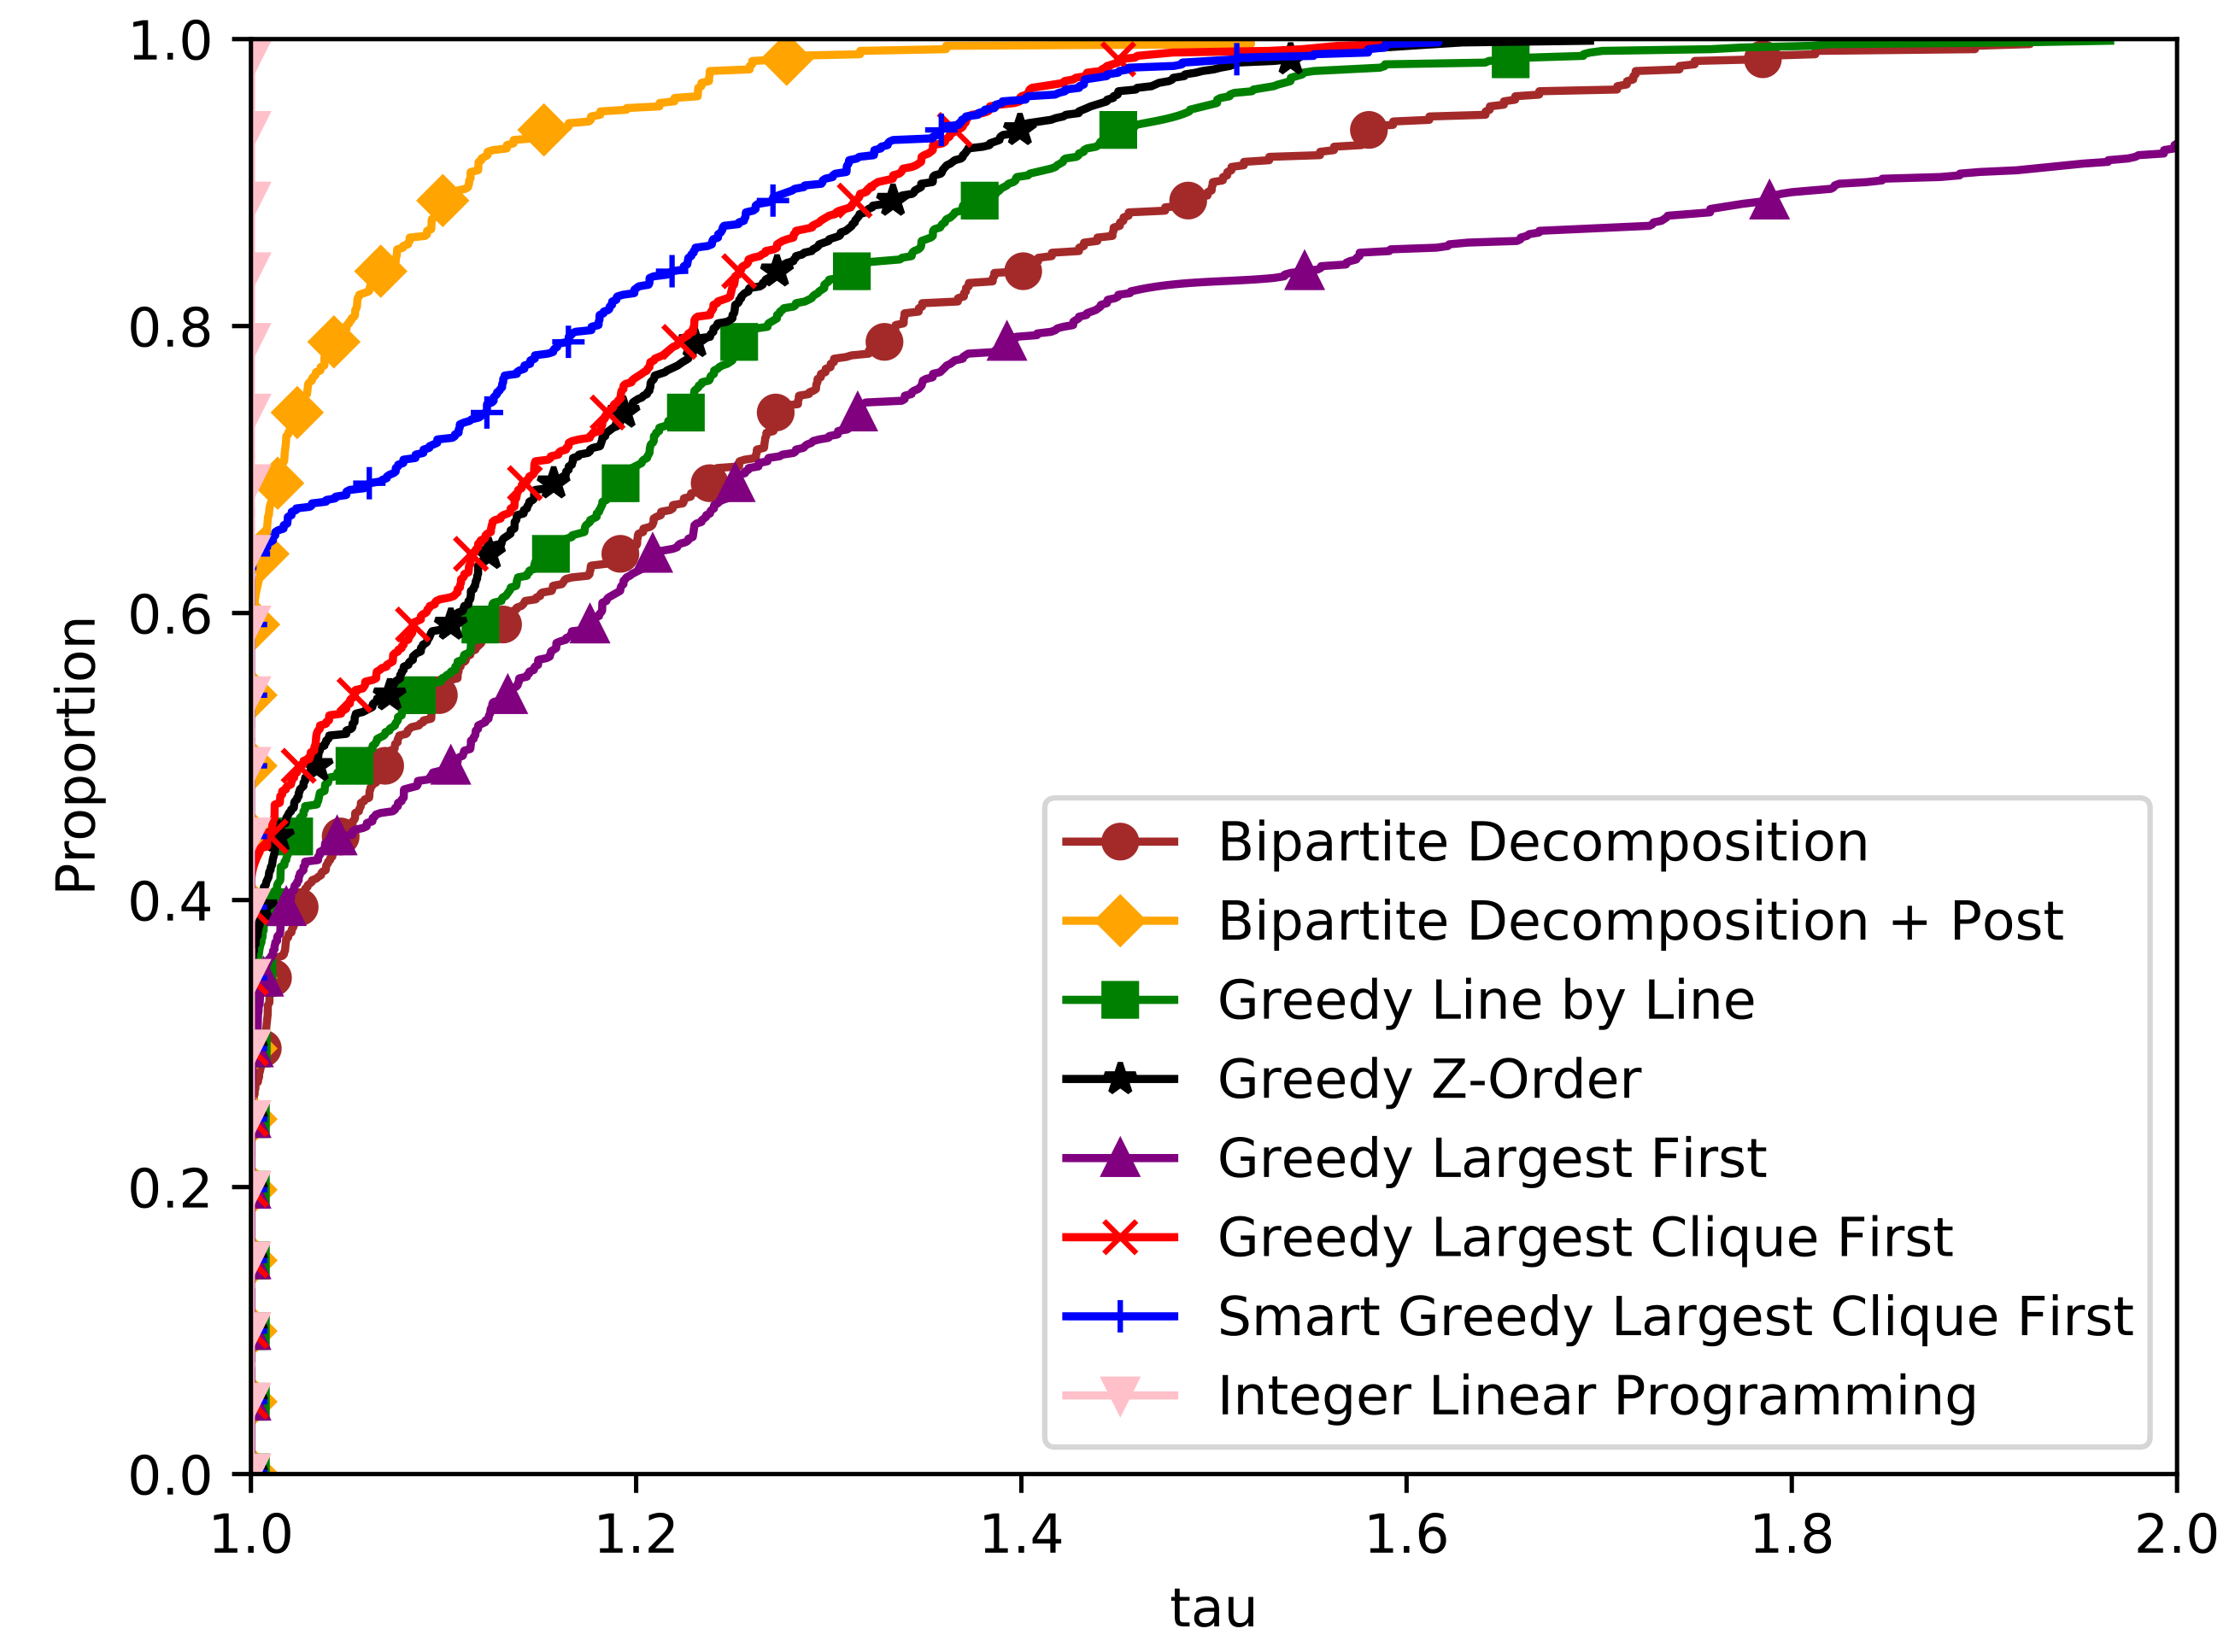
\includegraphics[width=0.4\textwidth]{figures/2d_results_ilp.png}
  \caption{2D Instances \cite{main_paper}.}
  \label{2d_results_ilp}
\end{figure}

\begin{figure}[h]
  \centering
  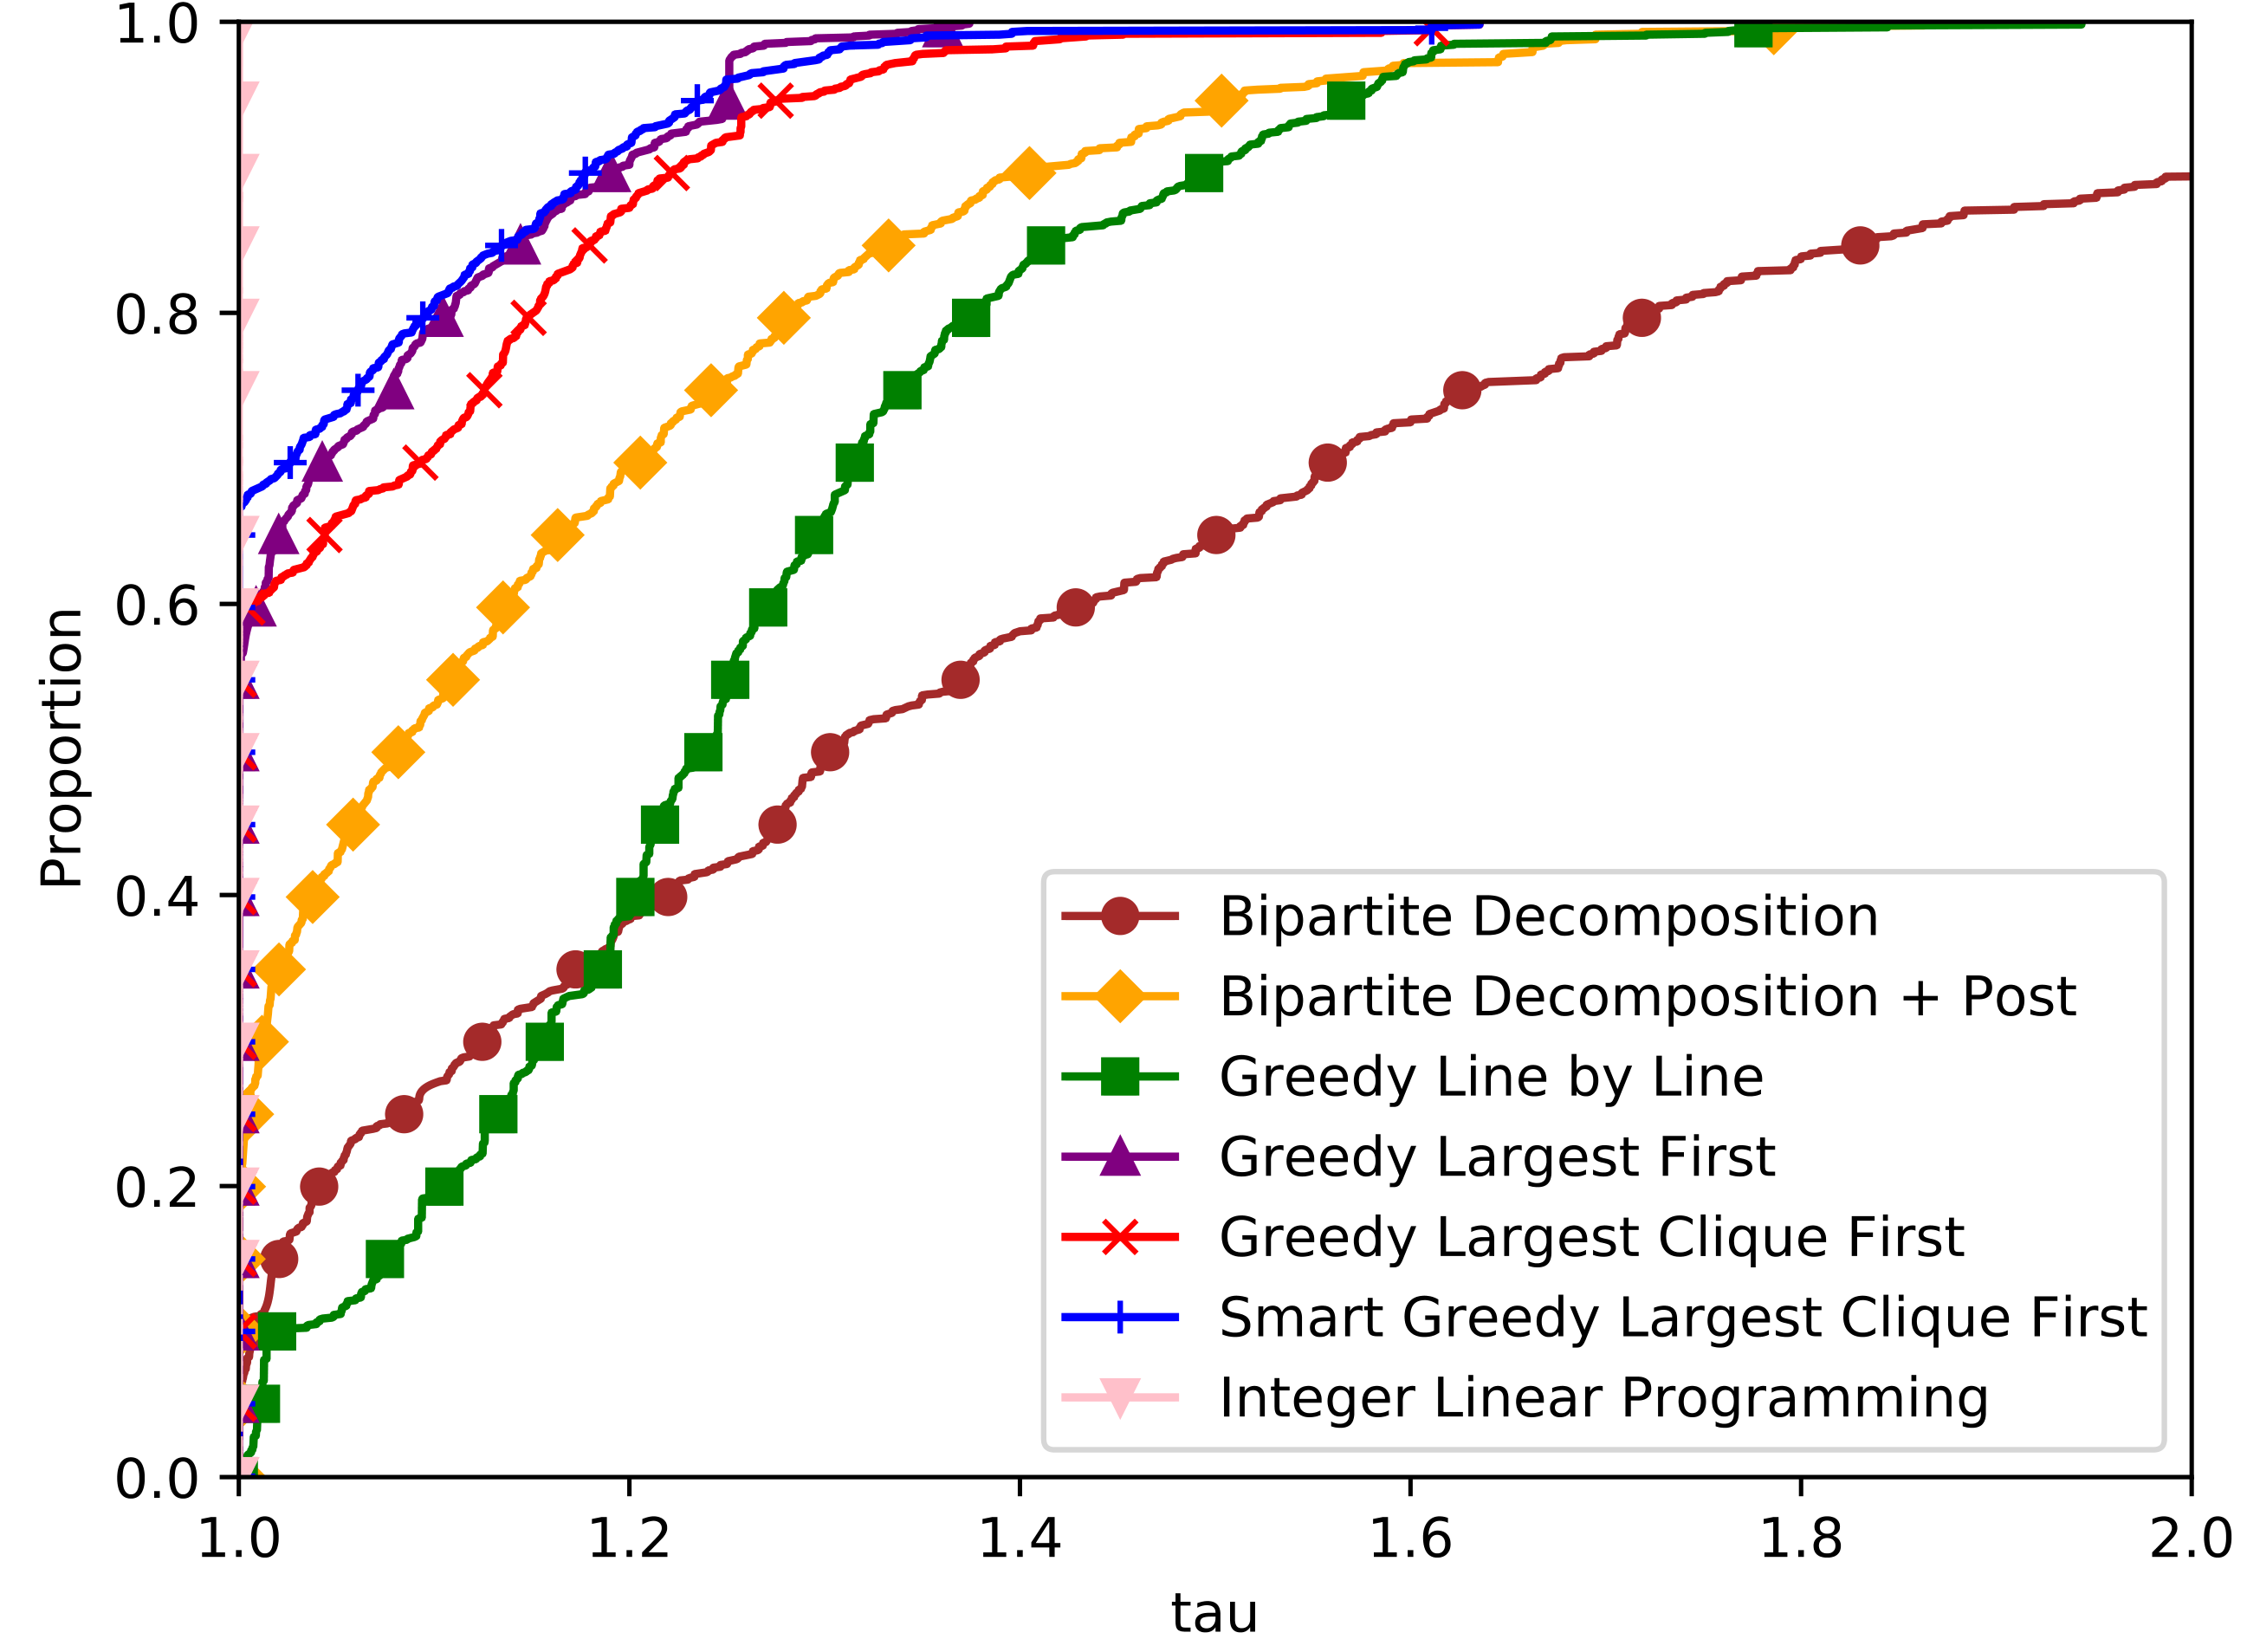
\includegraphics[width=0.4\textwidth]{figures/3d_results_ilp.png}
  \caption{3D Instances \cite{main_paper}.}
  \label{3d_results_ilp}
\end{figure}

\begin{figure}[h] 
  \centering
  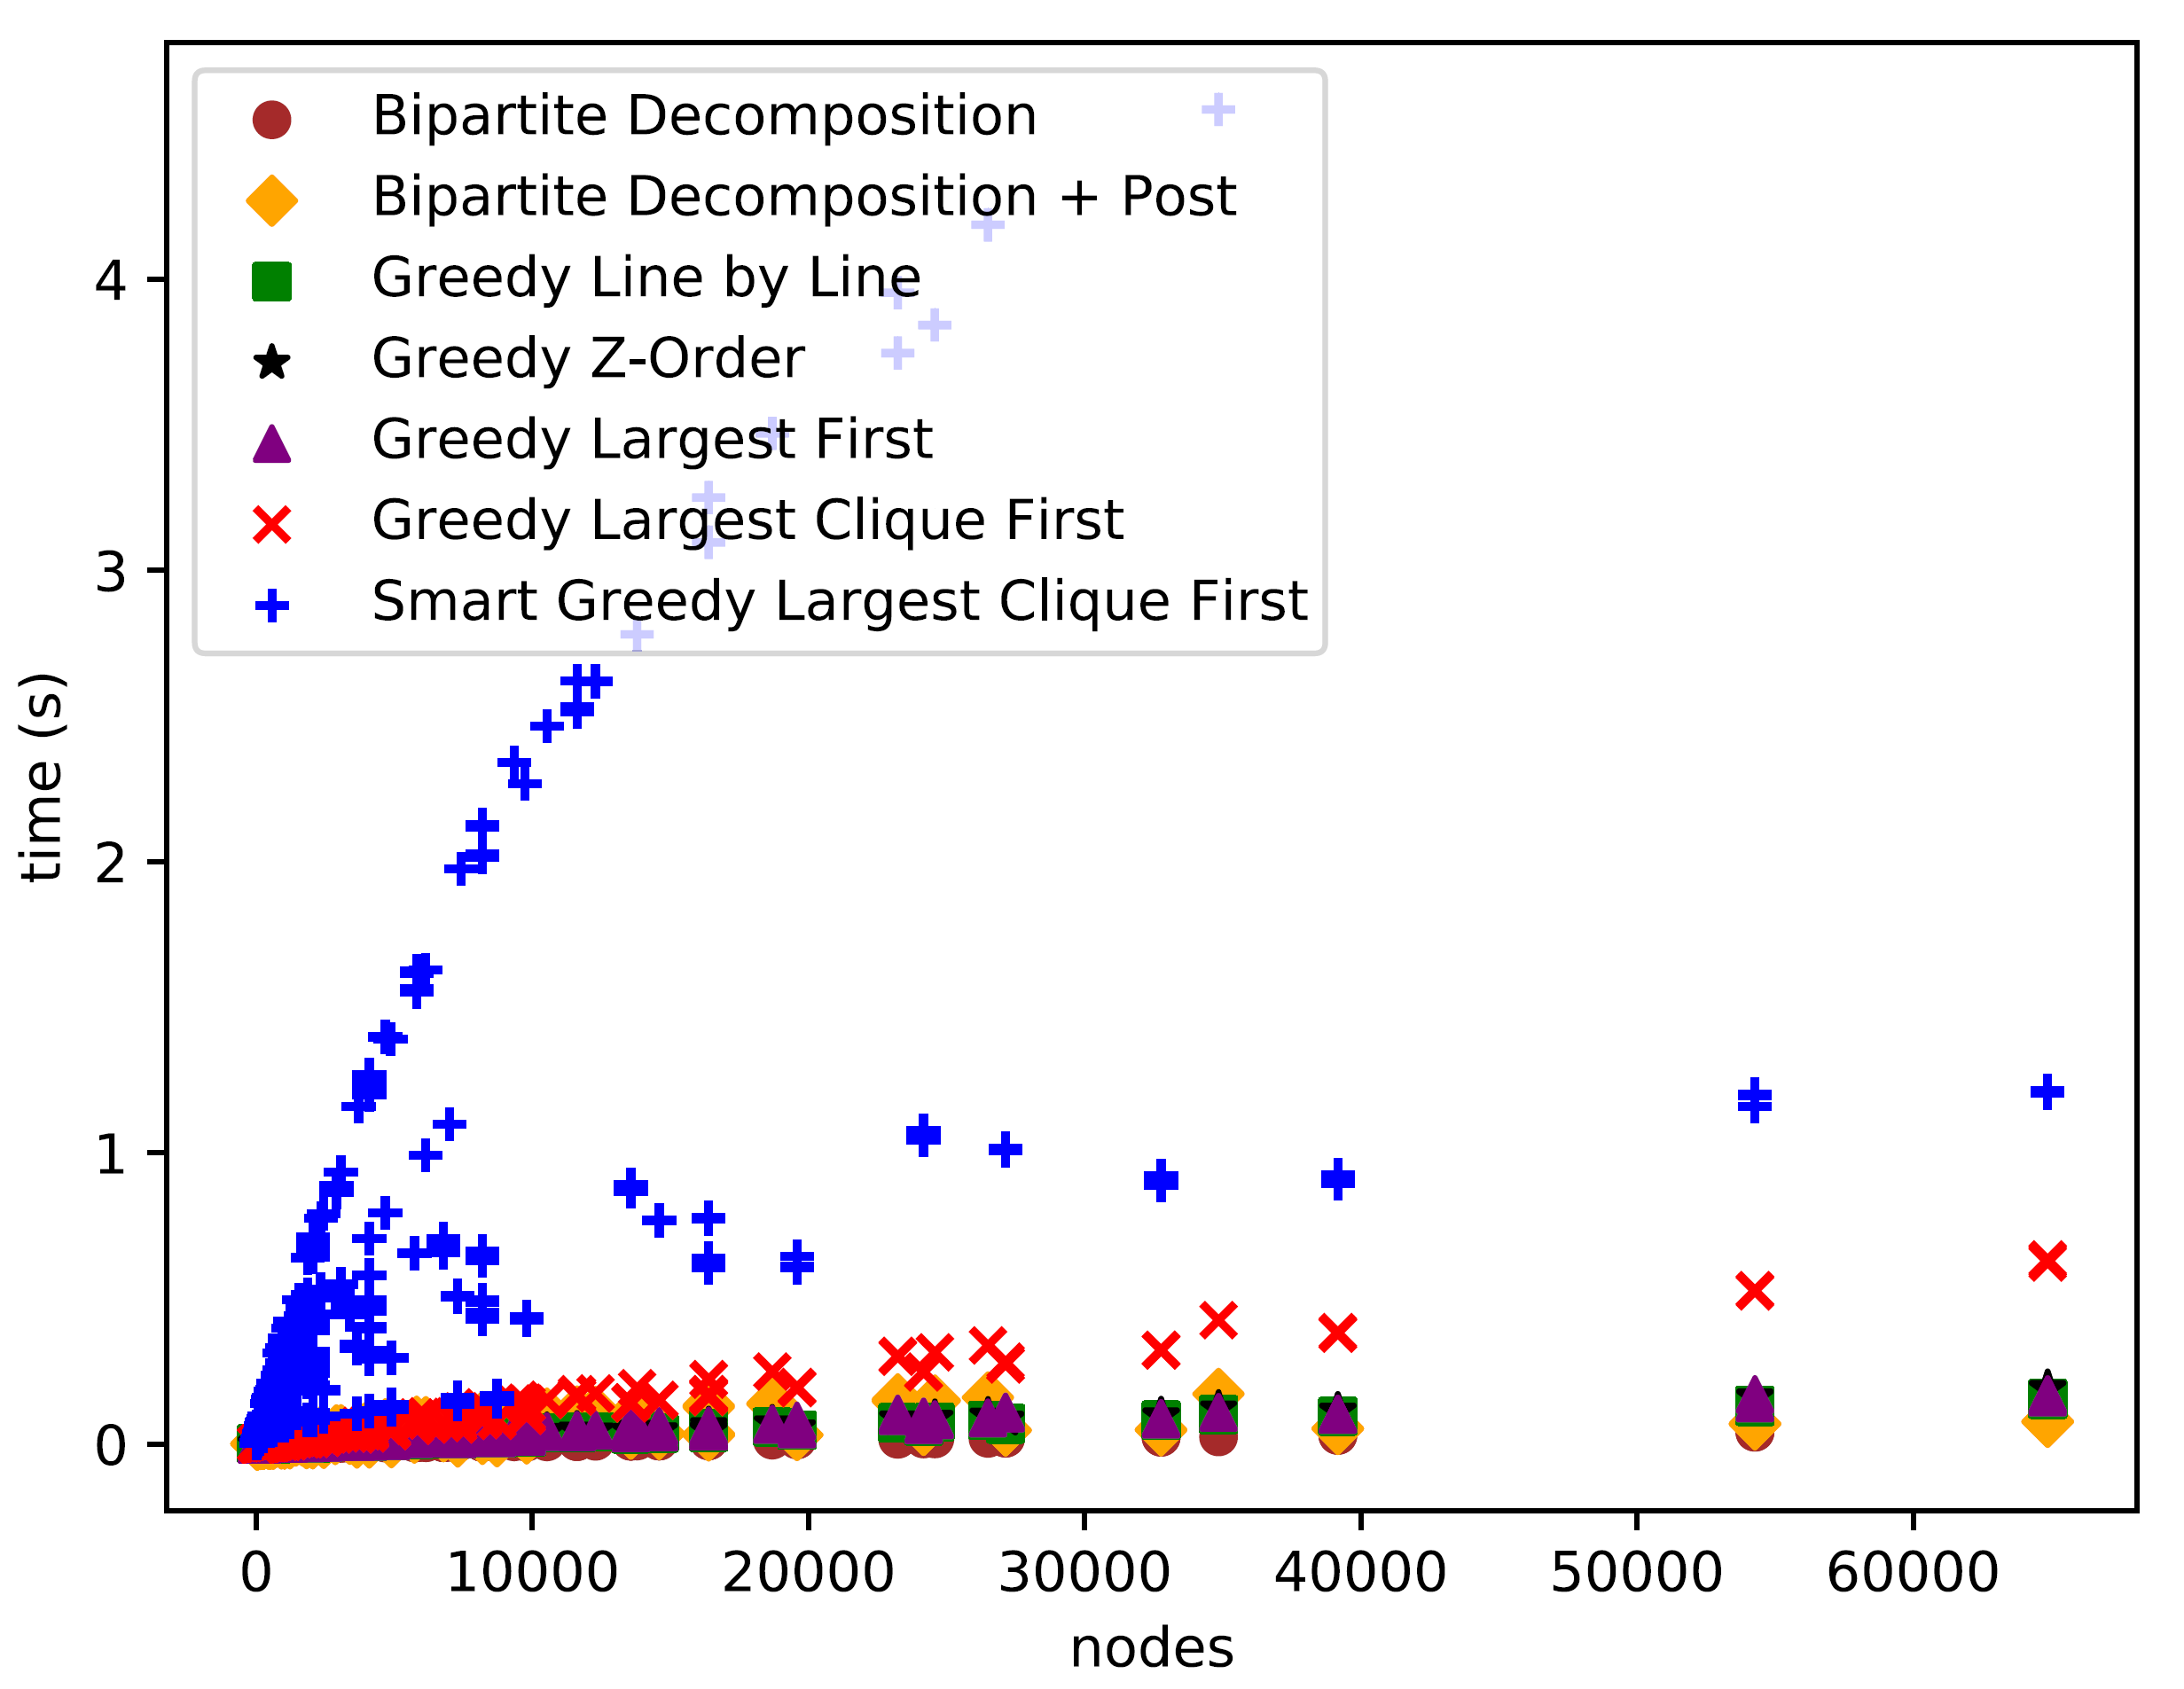
\includegraphics[width=0.4\textwidth]{figures/time_results_2D.png}
  \caption{Execution Time (ET) for coloring solution in 2D instances \cite{main_paper}.}
  \label{ET_2D}
\end{figure}

\begin{figure}[h]
  \centering
  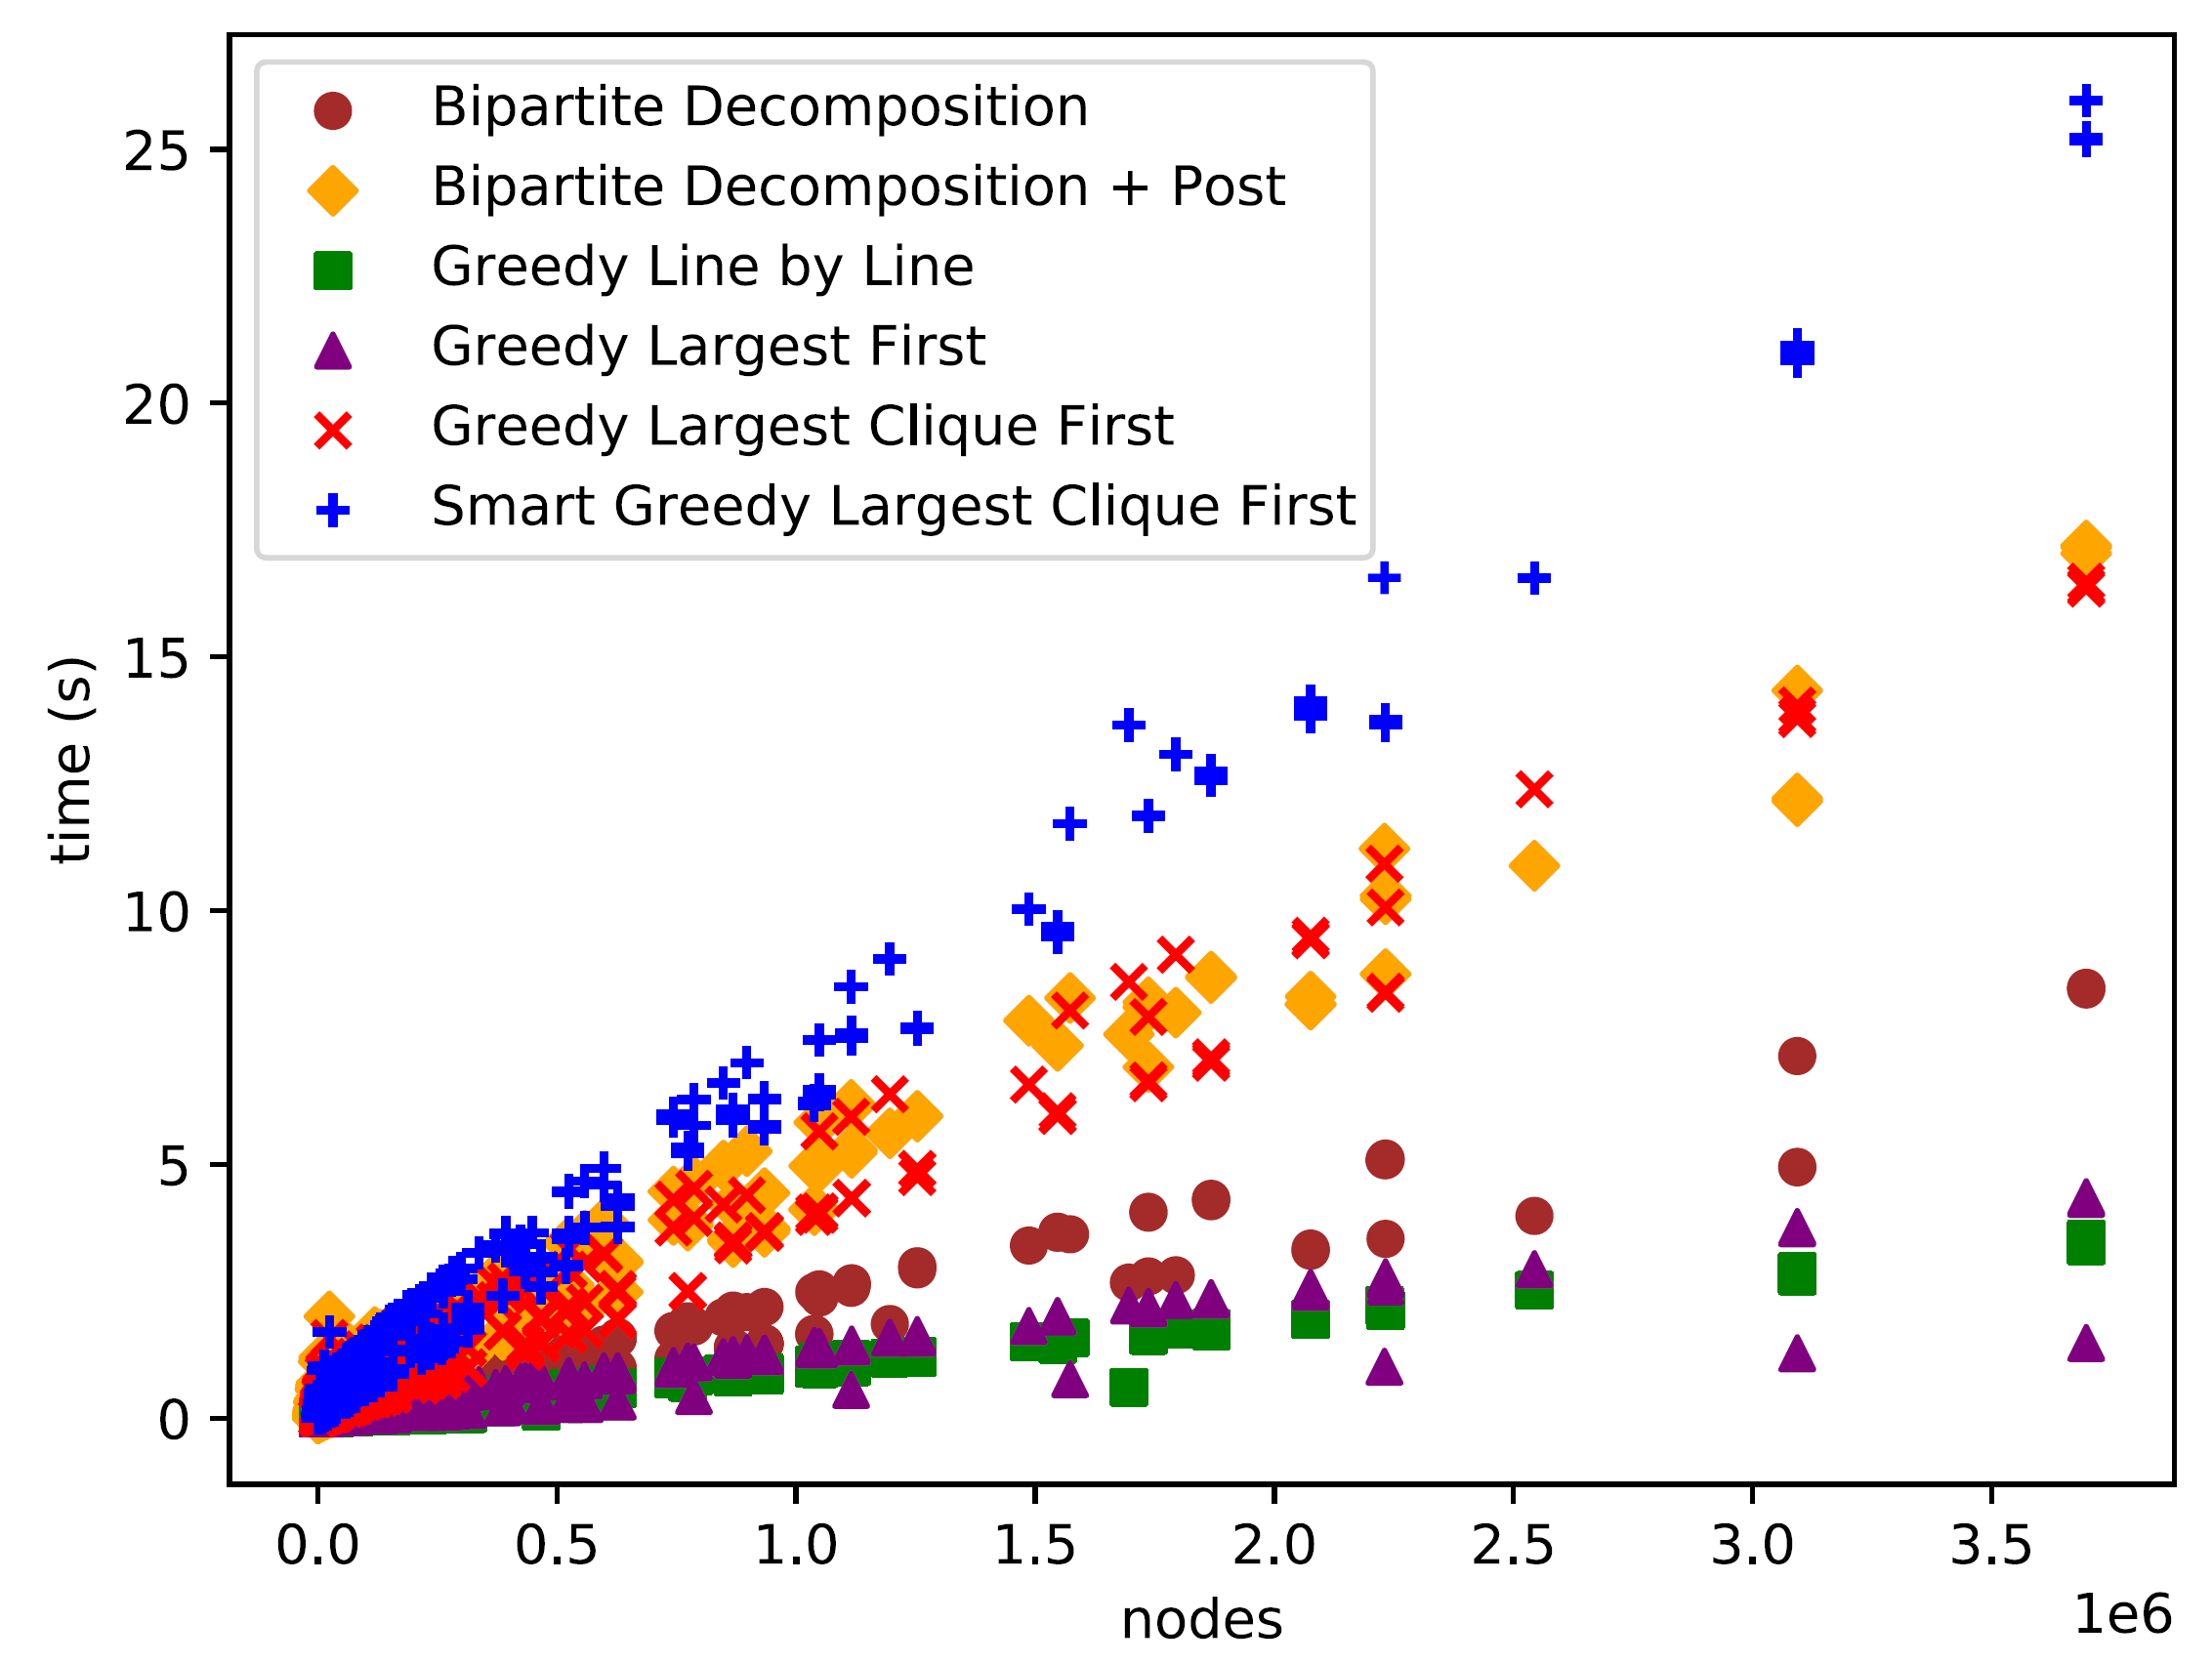
\includegraphics[width=0.4\textwidth]{figures/time_results_3D.png}
  \caption{Execution Time (ET) for coloring solution in 3D instances \cite{main_paper}.}
  \label{ET_3D}
\end{figure}

\section{Conclusion}
The authors have additionally proven the NP-Completeness of the Interval Vertex Coloring Problem for 3D stencils while
failing to deliver the proof for the 2D stencil case. While this critique seems harsh it is worth noting that 
the authors delivered algorithms that yield approximation solutions which were quite good, 90\% of the solutions only 1.2 times as bad as optimal solution, and are proven to run in linear time.
Nevertheless future work could contain the proof of the 2D case and extensions to graphs other than the 2D and 3D stencils.

\bibliographystyle{acm}
\bibliography{mybibliography}

\end{document}
